\documentclass[10pt,a4paper]{article}
\usepackage[utf8]{inputenc}
\usepackage[spanish]{babel}
\usepackage{amsmath}
\usepackage{amsfonts}
\usepackage{amssymb}
\usepackage[T1]{fontenc} 
\usepackage[left=3cm,right=3cm,top=3cm,bottom=3cm]{geometry}
\usepackage{acronym}
\usepackage{listings}
\usepackage{graphicx}
\graphicspath{ {images/} }
\usepackage{hyperref}

\usepackage{multirow}
\usepackage[table,xcdraw]{xcolor}

\usepackage[export]{adjustbox}
\usepackage{subcaption}


\title{
Práctica 3: Detección de puntos relevantes y Construcción de panoramas\\
\large Visión por Computador \\
}

\author{
Alejandro Palencia Blanco\\
}

\date{30/12/2020}

\begin{document}

\maketitle


\section{Ejercicio 1}

Este ejercicio se centra en la detección de puntos Harris sobre las imágenes Yosemite1 y Yosemite2. Posteriormente, se hace uso de la función drawKeyPoints() para su visualización. Para ello, he creado la función deteccionPuntosHarris() que tiene cinco parámetros: 
\begin{itemize}
	\item img: imagen sobre la que se detectan los puntos Harris
	\item block\_size: tamaño de ventana usado para extraer el criterio harris de cada píxel
	\item ksize: tamaño de máscara del operador de Sobel usado en el cálculo del criterio harris
	\item dist\_max: distancia entre máximos locales
	\item umbral: usado para descartar píxeles con criterio Harris por debajo de este valor
\end{itemize}

\subsection{Apartados a, b y c}
Empiezo creando la pirámide gaussiana que usaré para hallar los puntos Harris. Primero paso la imagen original a escala de grises (este será el primer nivel) y luego calculo los otros dos niveles usando la función pyrDown(). A continuación, para cada uno de los tres niveles de la pirámide, calculo los puntos Harris de la siguiente forma:
\begin{enumerate}
	\item Hallo los valores propios $\lambda_1$, $\lambda_2$ mediante la función cornerEigenValsAndVecs(). Para todos los niveles he usado un block\_size=5, ya que al fijarlo a 7 obtenía muy pocos puntos. Por otro lado, he usado un ksize=5, pues al fijarlo a 3 los puntos obtenidos también eran demasiado pocos. A continuación, a partir de los valores propios calculo el criterio Harris de cada píxel, es decir, $\lambda_1 \lambda_2 / (\lambda_1 + \lambda_2)$. Para evitar dividir por cero si ambos valores propios son cero, añado una constante despreciable a la suma del denominador (concretamente, $10^{-6}$).
	
	\item Calculo las derivadas parciales de la imagen haciendo uso del operador de Sobel. Primero, aplico un alisamiento gaussiano con sigma=4.5 usando la función GaussianBlur() y a la imagen resultante le aplico el operador de Sobel tanto en el eje X como en el eje Y. Esto último lo hago con la función Sobel(). Estas imágenes serán usadas más adelante para hallar los gradientes en cada píxel, los cuales a su vez nos permitirán calcular la orientación de cada punto Harris.
	
	\item Para cada píxel, aplico la supresión de no máximos para quedarme solo con aquellos píxeles que son máximos locales, los cuales serán los puntos harris. Para guardarlos, construyo por cada uno de ellos una estructura KeyPoint con cuatro parámetros: coordenadas x e y del píxel, escala y orientación. Para implementarlo, tomo una matriz auxiliar de booleanos que lleva la cuenta de los píxeles que quedan por reexplorar. En primer lugar, descarto todos aquellos píxeles cuyo criterio Harris esté por debajo del umbral fijado. A continuación, realizo los siguientes pasos para el resto de píxeles:
	\begin{enumerate}
		\item Tomo la ventana centrada en el píxel cuyo lado sea igual a dist\_max, la distancia entre máximos (si el píxel está muy cerca del borde de la imagen, tomo la ventana un poco más pequeña por la zona del borde de forma que ésta no se salga fuera de la imagen).
		\item Compruebo si el valor de criterio Harris del píxel central es el valor máximo de la ventana seleccionada. En caso negativo, solo marco el píxel central como explorado. En caso afirmativo, el píxel central es punto Harris, luego marco todos los píxeles de la ventana como explorados y paso a crear su estructura KeyPoint. Para el KeyPoint, especifico las coordenadas x e y (en el primer nivel de la pirámide, la imagen original), la escala (que será mayor cuanto mayor sea el nivel de la pirámide, concretamente $2^{nivel}block\_size$) y la orientación. Para calcular esto último, tomo los valores correspondientes al píxel central de las derivadas parciales obtenidas anteriormente con el operador de Sobel. Estos valores dan un gradiente, el cual normalizo y utilizo para hallar la orientación, que es el ángulo que forma con el eje X positivo. Si $(g_x,g_y)$ es el gradiente, entonces dicho ángulo es $\text{sgn}(g_y) \arccos (g_x)$ donde sgn es la función signo.
	\end{enumerate}
\end{enumerate}

En la práctica, se propone usar una distancia entre máximos que esté en el rango de 5 a 11 píxeles. Para valores mayores a 5 obtenía muy pocos puntos (ya que a mayor distancia entre máximos, menor será el número de puntos Harris que se espera obtener), así que he decidido tomar dist\_max=5. A continuación, he fijado un umbral muy bajo (en torno a $10^{-3}$) y lo he incrementado progresivamente hasta obtener un conjunto de puntos Harris que se encuentre razonablemente cerca de los 2000 y cuya proporción entre los tres niveles de la pirámide sea en torno a 70\%-25\%-5\%. Finalmente, el umbral con el que me he quedado ha sido 0.015.


\subsection{Apartado d}

Los puntos Harris que he obtenido en Yosemite1 son 2252 con una proporción de 77.66\% en el primer nivel (1749), 17.67\% en el segundo (398) y 4.66\% en el tercero (105). La imagen obtenida con drawKeypoints() es la siguiente:

\begin{figure}[h]
	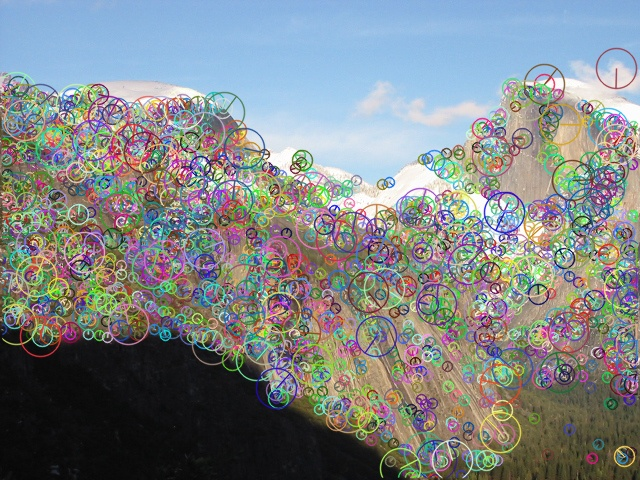
\includegraphics[width=\textwidth]{yosemite1_kpts}
\end{figure}


Los puntos Harris que he obtenido en Yosemite2 son 2027 con una proporción de 77.35\% en el primer nivel (1568), 17.76\% en el segundo (360) y 4.88\% en el tercero (99). La imagen obtenida con drawKeypoints() es la siguiente:

\begin{figure}[h]
	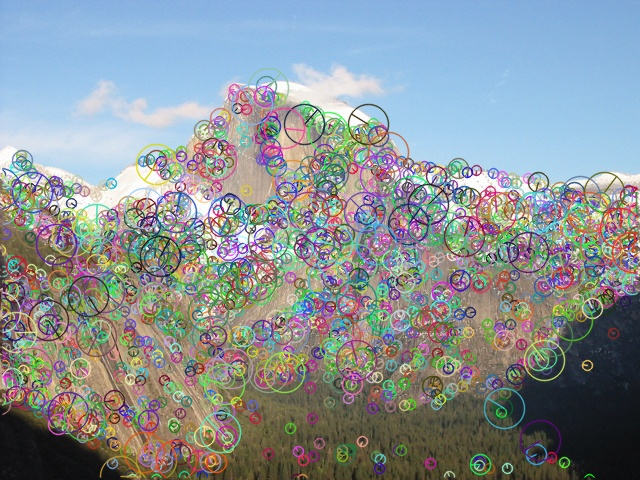
\includegraphics[width=\textwidth]{yosemite2_kpts}
\end{figure}

Vemos que en ambas imágenes, los círculos se concentran en las zonas de las montaña (como cabía esperar pues es donde hay más esquinas). Por el contrario, las zonas de cielo, de sombra o incluso de nieve, al ser muy planas, no tienen prácticamente ningún punto Harris. Por último, las zonas de bosque (en la parte inferior de las imágenes) tienen algunos puntos Harris, pero observamos que son pocos comparados con los de las montañas y que la mayoría tienen radios pequeños (es decir, corresponden a la octava más baja de la pirámide gaussiana). Por todo esto, considero que los puntos Harris que he calculado son coherentes con lo que se esperaba obtener.

\subsection{Apartado e}
En primer lugar, uso la función cornerSubPix para calcular las coordenadas subpixel de cada punto Harris. Para ello, extraigo de cada KeyPoint las coordenadas x e y del punto Harris y las coloco en una lista, la cual será el segundo parámetro de la función. También le paso la imagen original en escala de grises como primer parámetro y especifico que la mitad del tamaño de la región de búsqueda sea (3,3) para que la región de búsqueda del refinamiento sea 7x7. Por último, impongo que el criterio de parada sea tanto por un número máximo de 50 iteraciones como por un movimiento de la posición de la esquina inferior a un épsilon=0.01 en alguna iteración (lo que ocurra antes).

Una vez que tengo los puntos Harris refinados, selecciono tres de ellos aleatoriamente y muestro las imágenes interpoladas a un zoom 10x de los entornos 9x9 de dichos píxeles. La selección se hace evitando aquellos puntos demasiado cercanos al borde para poder dibujar una región 9x9 centrada en él. Una vez seleccionada la región 9x9, interpolo a un zoom 10x usando la función resize() y especificando que la ventana tenga tamaño 90x90. Sobre esta ventana, añado mediante la función circle() una marca azul sobre el punto Harris sin refinar y una marca roja sobre el punto refinado (si solo aparece una marca roja en el centro, significa que el refinamiento conincide con el punto sin refinar).

Los tres refinaminamientos subpixel obtenidos en Yosemite1 son los siguientes:

\begin{figure}[h]
\begin{subfigure}{0.33\textwidth}
	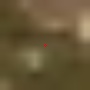
\includegraphics[height=90px,width=90px]{yosemite1_subpixel1}
\end{subfigure}
\begin{subfigure}{0.33\textwidth}
	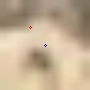
\includegraphics[height=90px,width=90px]{yosemite1_subpixel2}
\end{subfigure}
\begin{subfigure}{0.33\textwidth}
	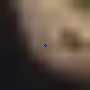
\includegraphics[height=90px,width=90px]{yosemite1_subpixel3}
\end{subfigure}
\end{figure}

Los tres refinaminamientos subpixel obtenidos en Yosemite2 son los siguientes:

\begin{figure}[h]
	\begin{subfigure}{0.33\textwidth}
		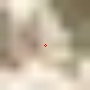
\includegraphics[height=90px,width=90px]{yosemite2_subpixel1}
	\end{subfigure}
	\begin{subfigure}{0.33\textwidth}
		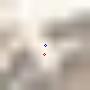
\includegraphics[height=90px,width=90px]{yosemite2_subpixel2}
	\end{subfigure}
	\begin{subfigure}{0.33\textwidth}
		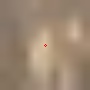
\includegraphics[height=90px,width=90px]{yosemite2_subpixel3}
	\end{subfigure}
\end{figure}

Vemos que algunos refinamientos han modificado la posición original del punto Harris mientras que otros permanecen igual.



\newpage
\section{Ejercicio 2}

En este ejercicio se pide primero detectar los keypoints y extraer los descriptores AKAZE para las imágenes Yosemite1 y Yosemite2 y luego establecer correspondencias entre los keypoints extraidos en ambas imágenes. Para ello, he creado la función correspondenciasAKAZE(), que recibe como parámetros las dos imágenes sobre las que se establecerán correspondencias. Lo primero que hace esta función es pasar ambas imágenes a escala de gris y detectar los keypoints y extraer los descriptores AKAZE. Para ello, creo un objeto AKAZE que desempeñe esta tarea mediante AKAZE\_create() y a continuación llamo al método detectAndCompute() para obtener los keypoints y los descriptores AKAZE de cada imagen.

Una vez tengo los descriptores, podemos establecer correspondencias creando un objeto de tipo BFMatcher, el cual es un emparejador de descriptores que para cada descriptor de la primera imagen encuentra el descriptor más cercano de la segunda imagen por fuerza bruta (es decir, intentando emparejar uno por uno). Al crearlo mediante la función BFMatcher\_create(), especifico que la norma sea la euclídea y que se use el criterio crossCheck, el cual asegura que en cada correspondencia, el descriptor de la segunda imagen también está emparejado con el descriptor más cercano de la primera imagen, es decir, solo se devuelven parejas consistentes. Normalmente este criterio produce resultados con un menor número de outliers o falsas correspondencias. Para obtener estas correspondencias, simplemente llamo al método match() del emparejador.

Para terminar, esta función aplica el criterio de Lowe del segundo vecino más cercano (Lowe 2-NN) y devuelve tanto las listas de keypoints de cada imagen como las correspondencias entre los mismos. Para implementar este otro criterio, he creado otra funcion llamada criterioLowe2NN(), que toma como parámetros los descriptores de cada imagen, las correspondencias y un ratio (que será un número entre 0 y 1, 0.7 por defecto). Primero, creo una matriz en la que almaceno, para cada pareja de descriptores (uno de la primera imagen y otro de la segunda), su distancia euclídea. Luego, en cada correspondencia, tomo para el descriptor de la primera imagen aquel descriptor de la segunda cuya distancia al primero sea la segunda menor (es decir, el segundo vecino más cercano). A partir de esta distancia, descarto la correspondencia si cociente de distancias al vecino más cercano y al segundo vecino más cercano es mayor que el ratio (pues esto significa que la segunda mejor opción es casi tan buena como la primera, luego descartamos la correspondencia por ser ambigua). Este mismo procedimiento también lo realizo en el otro sentido, es decir, hallando para los descriptores de la segunda imagen sus segundos vecinos más cercanos en la primera.

Después de llamar a la función anteriormente descrita, he obtenido 495 correspondencias antes de aplicar el criterio Lowe 2-NN y 342 después de aplicarlo. Con las correspondencias ya extraídas, creo un par de ejemplos en los que selecciono de forma aleatoria cien correspondencias y muestro ambas imágenes en un mismo canvas pintando segmentos entre los puntos en correspondencia. Los resultados son los siguientes:

\begin{figure}[h]
	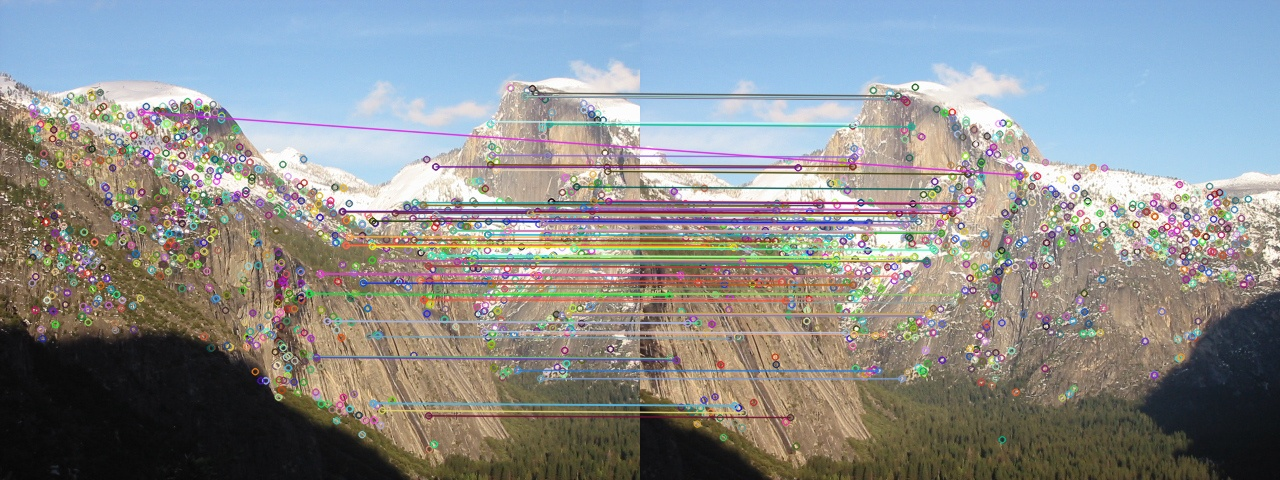
\includegraphics[width=\textwidth]{corresp1_yosemite}
\end{figure}

\begin{figure}[h]
	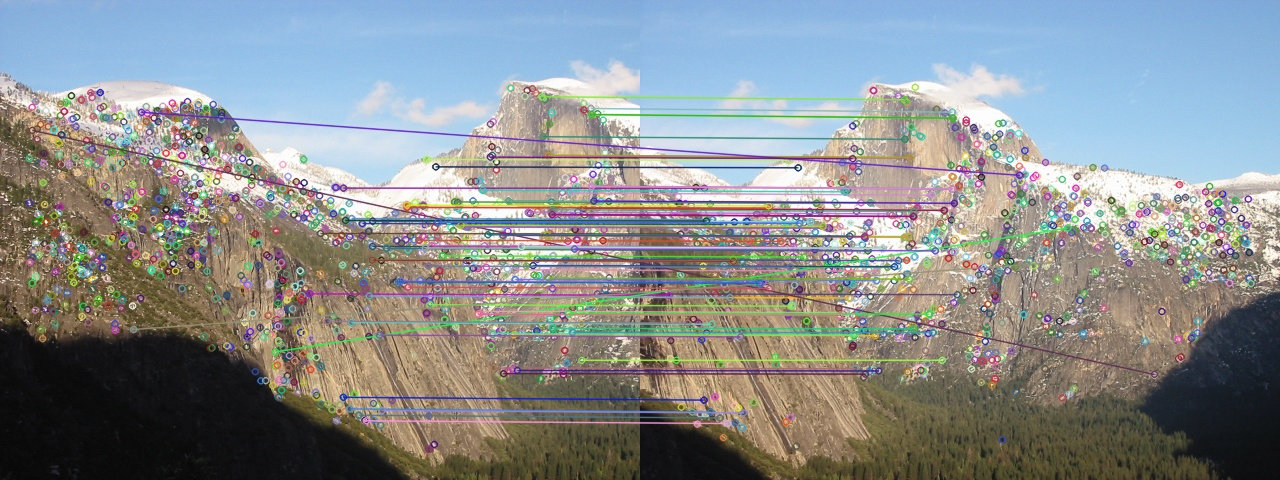
\includegraphics[width=\textwidth]{corresp2_yosemite}
\end{figure}

\newpage
Si observamos ambas imágenes antes de realizar todo este proceso, podemos deducir que la imagen Yosemite2 ha sido tomada aplicando una traslación horizontal hacia la derecha con respecto a Yosemite1. Por tanto, es esperable que los puntos en correspondencia muestren segmentos horizontales en el canvas, todos ellos con longitudes casi idénticas. Los canvas obtenidos dejan ver que la gran mayoría de estas correspondencias dibujan precisamente este tipo de segmentos, salvo un pequeño subconjunto de éstas, las cuales dibujan segmentos con cierta inclinación fácilmente detectables. No es difícil ver que estas últimas correspondencias son falsos positivos. A pesar de ellos, considero que los resultados obtenidos son bastante buenos, pues la proporción de falsos positivos con respecto al total de correspondencias encontradas parece ser muy baja atendiendo a la información arrojada por los canvas. Algoritmos como RANSAC pueden trabajar sin problema con este tipo de conjuntos en los que hay algunos outliers pero el conjunto de inliers es suficientemente numeroso.






\newpage
\section{Ejercicio 3}

Para este ejercicio he diseñado una función llamada mosaico3Imagenes() que recibe como parámetros las tres imágenes usadas para construir el mosaico y devuelve el mosaico construido mediante homografías. La detección de keypoints y extracción de descriptores AKAZE y el cálculo de correspondencias se hace de forma idéntica a como se ha hecho en el ejercicio 2.

Para encontrar las homografías que me permitan llevar puntos de una imagen a otra, uso la función findHomography(), la cual toma como parámetros las coordenadas de cada pareja de puntos en correspondencia. Estas coordenadas las agrupo en dos listas según pertenezcan a la imagen de origen o a la imagen de destino. También especifico que la homografía sea calculada usando RANSAC, un algoritmo iterativo diseñado para excluir los outliers en el cálculo de ésta. 

Para intentar que el mosaico obtenido tenga la mayor calidad posible, procedo de la siguiente forma:
\begin{itemize}
	\item Eligo una imagen del centro como base para calcular el mosaico. Esta imagen será llevada al centro del mosaico mediante una homografía que simplemente consistirá en una traslación, la cual llamaré $H_0$.
	\item Se calculan las homografías que van de la imagen de la izquierda a la central, $H_{1,2}$, y de la derecha a la central, $H_{3,2}$. Después, compongo dichas homografías con $H_0$ para obtener $H_1 = H_0 \circ H_{1,2}$ y $H_3 = H_0 \circ H_{3,2}$, respectivamente. Estas últimas son las que usaré para llevar las imágenes de la izquierda y de la derecha al mosaico.
	\item Por último, coloco primero en el mosaico aquellas imágenes que necesitan un mayor procesamiento para ser llevadas al mismo, es decir, aquellas cuya homografía asociada se obtiene por composición de un mayor número de homografías. En este caso, estas imágenes son la de la izquierda y la de la derecha. La de centro será la última en ser colocada. Al seguir este orden, consigo que partes de las imágenes con menor calidad queden solapadas por imágenes con mayor calidad, luego en general el mosaico también mejora ligeramente.
\end{itemize}

Originalmente, el mosaico es un array con altura y anchura suficientemente grandes como para que quepan todas las imágenes que se quieren colocar en él. Una vez se tiene para cada imagen la homografía que la coloca en el mosaico, éste se construye mediante la función warpPerspective(), especificando que el borde sea de tipo BORDER\_TRANSPARENT para que al colocar sucesivas imágenes no se borren aquellas que se han colocado anteriormente.

Este es el mosaico que he obtenido:

\begin{figure}[h]
	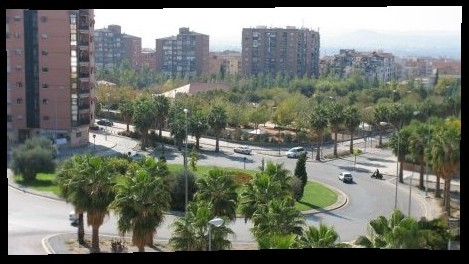
\includegraphics[width=\textwidth]{mosaico3Imgs}
\end{figure}

Podemos ver que el resultado final es bastante realista, salvo por algunas zonas en las que hay objetos en movimiento. Por ejemplo, en la esquina inferior izquierda se puede ver un coche blanco detrás de unas palmeras del cual solo se muestra la parte de atrás. Esto ocurre porque, al estar las fotos tomadas en distintos momentos, el coche aparece en la imagen de la izquierda pero no en la central, lo cual provoca que la parte delantera del mismo no aparezca al solapar la imagen central sobre la imagen de la izquierda. Este fenómeno pone de manifiesto que este procedimiento para construir mosaicos necesita que los objetos que aparecen en las fotos permanezcan estáticos mientras que éstas son tomadas, pues en caso contrario no es posible asegurar que el resultado que se va a obtener es satisfactorio.



\newpage
\section{Ejercicio 4}

Este ejercicio es una generalización del ejercicio anterior para un número arbitrario de imágenes ordenadas de derecha a izquierda. Por tanto, la función que he diseñado, mosaicoNImagenes(), tomará como parámetros una lista de $N$ imágenes y trabajará de forma muy similar a como lo hace la función del ejercicio anterior.

En esencia, esta función considera tres subconjuntos de imágenes: la imagen central, las imágenes que están a la izquierda de la central y las que están a la derecha de la central. Primero, se detectan los keypoints y se extraen los descriptores AKAZE y se establecen correspondencias entre pares de imágenes consecutivas tal y como se ha hecho anteriormente. A continuación, calculo las homografías entre pares de imágenes consecutivas desde la imagen que está más alejada de la central hacia la que está más cercana a ésta. Es decir, si el par de imágenes se encuentra a la izquierda de la central, calculo la homografía desde la que se encuentra más a la izquierda hacia la otra, y análogamente para las que se encuentran a la derecha. También calculo, al igual que antes, la homografía $H_0$ que traslada la imagen central al centro del mosaico.

A partir de aquí, ya se pueden calcular las homografías asociadas al resto de imágenes. Para calcular las que llevan las imágenes de la izquierda al mosaico, procedo de forma recursiva: si $\{H_{1,2},H_{2,3}\dots,H_{k-1,k}\}$ son las homografías asociadas a pares de imágenes consecutivas en la izquierda, siendo la primera imagen aquella que está más a la izquierda y la k-ésima imagen la central, entonces $H_{k-1} = H_0 \circ H_{k-1,k}$ y $H_{i} = H_{i-1} \circ H_{i-1,i}$ para todo $i \in \{1,\dots,k-2\}$. Para las imágenes de la derecha el cálculo es análogo.

Finalmente, solo queda colocar las imágenes en el mosaico. El orden también será análogo al anteriormente descrito: primero las imágenes de la izquierda, luego las de la derecha y por último la central. Tanto las imágenes a la izquierda como a la derecha se ordenan según su distancia a la imagen central, de mayor a menor, y en ese orden son colocadas en el mosaico.

El mosaico obtenido es el siguiente:

\begin{figure}[h]
	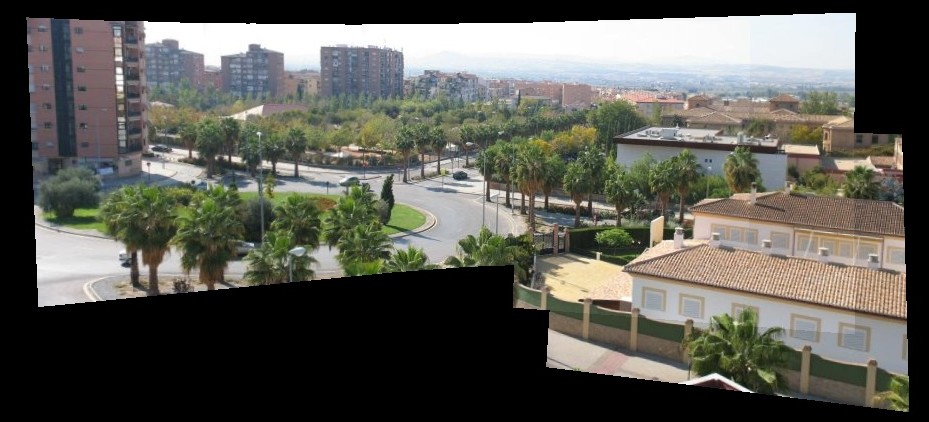
\includegraphics[width=\textwidth]{mosaicoNImgs}
\end{figure}

Además del fenómeno expuesto en el ejercicio anterior, vemos que en este mosaico también hay ligeros problemas relacionados con la fotometría. Más concretamente, en algunas zonas como el cielo o las paredes y los tejados de las casas (a la derecha del mosaico) podemos observar que hay cambios bruscos en la intensidad de los colores en las fronteras de imágenes solapadas. Al tomar las imágenes en distintos momentos, es posible que haya cambios en la luminosidad que provoquen este fenómeno, el cual puede ser resuelto mediante distintas técnicas de blending. Sin embargo, desde el punto de vista geométrico, se puede apreciar que las homografías permiten constriur panoramas sin ningún tipo de problema.



\end{document}



